\newcommand\prooftwo{
We construct the following NFA. Make new with x for match.
More formally,
\\
\begin{definition}[Deterministic Finite Automaton (DFA)]
A \textbf{finite automaton} is a 5-tuple $(Q, \Sigma, \delta, q_0, F)$, where
\begin{enumerate}
\item $Q$ is a finite set called the \textbf{states},
\item $\Sigma$ is a finite set called the \textbf{alphabet},
\item $\delta:\  Q\times \Sigma \rightarrow Q$ is the \textbf{transition function},
\item $q_0 \in Q$ is the \textbf{start state},
\item $F \subseteq Q$ is the \textbf{set of accept states}.
\end{enumerate}
\end{definition}
\\


\\
\begin{figure} \label{fig:dfastar}
    \centering
    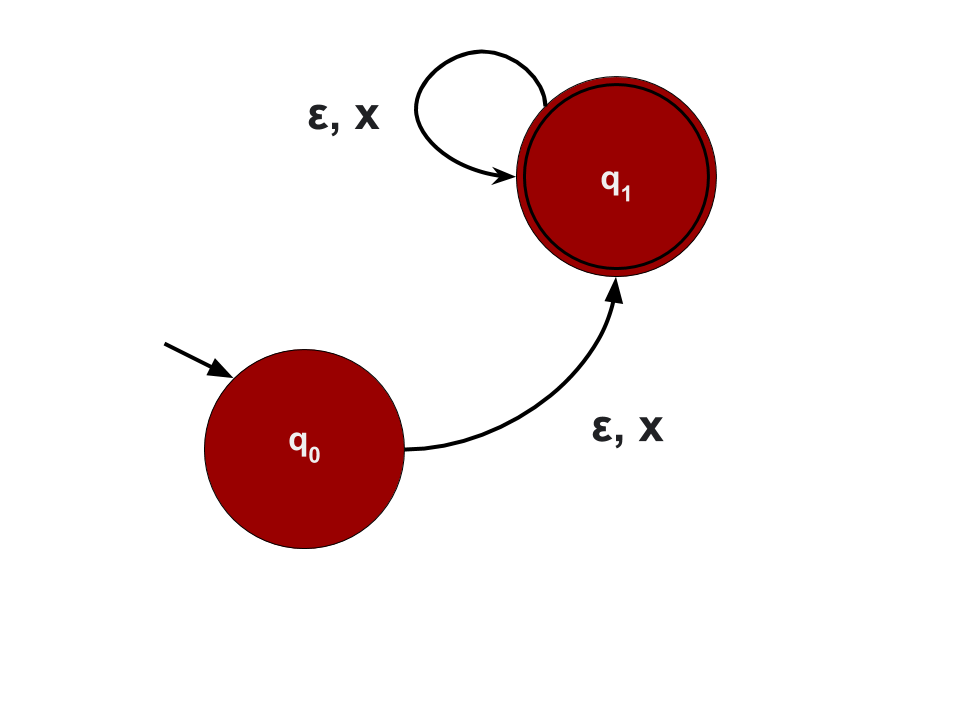
\includegraphics[width=0.75\linewidth]{Proofs/NFAQ2.png}
    \caption{NFA recognising $L^{*}$}
    \label{fig:my_label}
\end{figure}
\\

So the DFA in \ref{fig:dfastar} is formally $Q=\{q_{0},q_{1}\}$




Consider generally a language $L$ from the class of languages described by regular expressions. By Kleene's theorem (!proof i think?), we are just in considering 
\\$L:=\left\{ w\  |\  w\  is\  accepted\  input\  for\  some\  DFA\right\}  $
\\
instead, because the classes of regular languages are equivalent. The regular languages are precisely those which contain a finite number of strings, and for which some DFA can exist, able to process each string (via its transition function) from the start state to an (?caref myb NFA if so do equiv) accept state. We know, if $R$ is a regular expression, R (check! need to do all 6? probs) is $a$ for some $a$ in the alphabet $\Sigma$. Construct proof NFA that accepts concatations of multiple strings, this is all this new kleene star is doing (then go through all 6 reg expressions?). This is a subset (but not proper) of the regular languages, because regular expressions R has L(R) closed by Kleene. I think just draw the NFA for kleene star.(problem if x has length 5 (or something like cong 4p+1)? because 5 lots is square number --> that language is not reg or CFL?)  


\\
Shitbelow
\\
For each individual string $x \in L$, beacuse $L$ is described by a  regular expressions $L$ is a regular languages (Kleene's theorem). Thus, we can construct a DFA which accepts $x$, and label this $M_{1}$. Because the finite union of regular languages is closed, we can construct the following DFA to recognise every string $w=x....x$ for any finite number of $x$. Because this machine can recognise regular languages of the form $x=1$, we see in the case of $1^{n} n is square$, this is n 



The class of languages described by. Furthermore, if R is a regular expresision (R*) is a regular expression, by definition: this is  



Firstly consider the case w=x =. By definition x must be a regular expression. By Kleene's theroem then, x in L is a regular language, furthermore if zero copies, w=epsilon, which is fine because NFA is equiv to dfa so just swap all transition functions with input w=x for w=eps. Next we iterate, and we see we stay reg lang can't make xontext free. (Maybe use iteration fron a^n on complements, shrinking until just {a})







Consider the language \[ L :&= \{a^n b a^m \ | \ 1 \leq n \ \ \ \  0 \leq m \leq n \} \]
 \[ &= \{a^{p-1} {ba}^{m} \ | \ 1 \leq p  \ \ \ \ 1 < {m+1} \leq p \} \]
 \\
composed of finite-length strings w . Each string is composed of symbols xx,x in the alphabet gam. and thus we arrive \\

$Claim:\  If\  B\  is\  a\  language\  over\  the\  alphabet\  \Sigma ,\  then\  B=B^{+}\  iff\  BB\  \subseteq B.$
\\
$If\  R\  is\  a\  regular\  expression,\  L\left( R\right)  \  is\  the\  language\  of\  R.$
$All\  strings\  w\in R^{+}\  are\  1\  or\  more\  conatenations\  of\  strings\  from\  R.$
$All\  strings\  w\in R^{*}\  are\  0\  or\  more\  conatenations\  of\  strings\  from\  R.$
$i.e.$ \ $R^{+\  }\cup \  \epsilon \  =\  R^{\ast }$
\\
 More generally, if $\Sigma$ is any alphabet, the regular expression $\Sigma$ describes the language consisting of all strings of length 1 over this alphabet, and $\Sigma^{*}$ describes the language consisting of all strings over that alphabet. \\
 
}